\section{Kendall Correlation Coefficient}
\subsection{Background}
\subsubsection{Independence}
Two random variables $X$ and $Y$ are independent if and only if, for any two sets of real numbers, $A$ and $B$, 
\[\P (X \in A, Y \in B) = \P(X \in A) \P(Y \in B)\]

Equivalently, $X$ and $Y$ are independent if and only if 
\[F_{X, Y} (x, y) = F_X(x)F_Y(y)\]

Independent means that knowing the value of one does not change the distribution of the other.

Random variables that are not independent are said to be dependent.

In practice, we usually decide the dependence by common sense and prior knowledge, instead of the definition. Then the definition and properties are applied to the model.

\subsubsection{Correlation}
If $X$ and $Y$ are jointly distributed random variables with expectations $\mu_X$ and $\mu_Y$, respectively. The covariance of $X$ and $Y$ is \[\Cov(X, Y) = \E[(X - \mu_X)(Y-\mu_Y)].\]

If $X$ and $Y$ are independent, then $\Cov(X, Y) = 0$. But the converse is not necessary to be true. There could be non-linear relationship between $X$ and $Y$.

Suppose $\Var(X)$ and $\Var(Y)$ are both non-zero. The correlation of $X$ and $Y$ is \[\Corr(X,Y) \equiv \rho = \frac{\Cov(Y, Y)}{\sqrt{\Var(X)\Var(Y)}}\]

\subsubsection{Pearson Correlation Coefficient}
The definition of correlation is about random variables. Now suppose we have a data with sample size $n$. Then the sample correlation is actually the \textbf{Pearson Correlation Coefficient}
\[
\frac
{\sum_{i=1}^{n}
	(X_i - \bar{X})
	(Y_i - \bar{Y})
}
{\sqrt{
		\sum_{i=1}^{n}(X_i - \bar{X})^2 
		\sum_{i=1}^{n}(Y_i - \bar{Y})^2
	} 
}
\]

The Example R code is as follows. Note that for Person correlation, the hypothesis test is based on $t$-distribution.

\lstinputlisting[language=R]{code/pearson.R}


\begin{figure}[H]
	\centering
	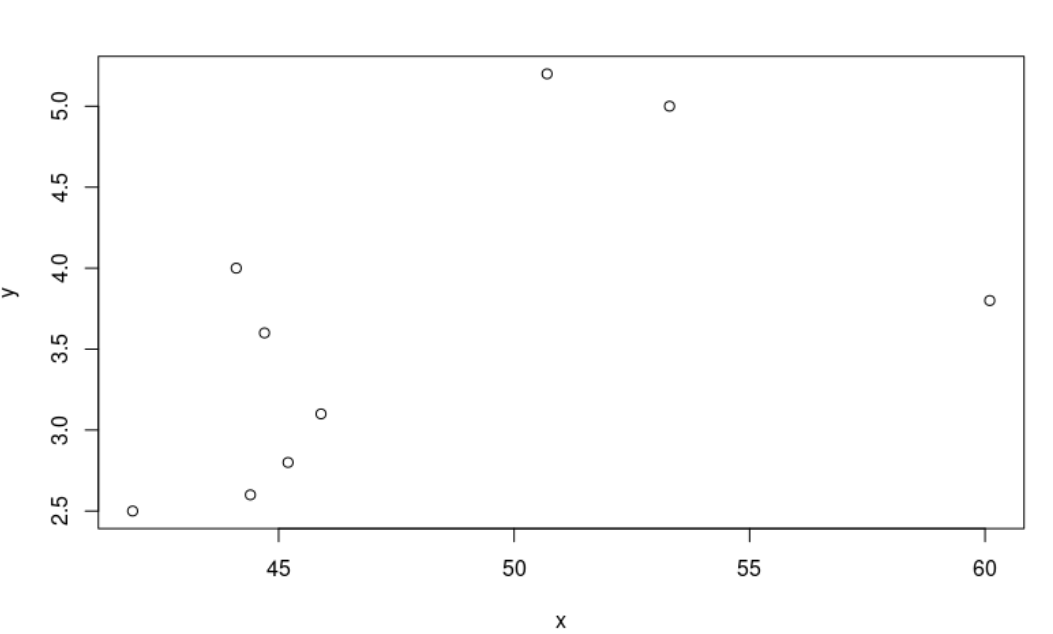
\includegraphics[width=0.7\linewidth]{fig/pearson}
	\caption{Dot Plot in Peason Example}
	\label{fig:pearson}
\end{figure}


\subsection{Assumption}
We suppose that the Data is a random sample from a bivariate population with $n$ subjects,
\[(X_1, Y_1), \cdots, (X_n, Y_n).\]

We look for the statistical relationship between the two variables in the bivariate structure.
\begin{itemize}
	\item Whether the two variables are independent.
	\item If not independent, what are the type and degree of dependency.
\end{itemize}

Assume $(X_1, Y_1), \cdots, (X_n, Y_n)$ are a random sample from a continuous bivariate population. That is $(X_i, Y_i)$ iid from a continuous bivariate distribution.

\subsection{Kendall Correlation Coefficient}
Suppose we have
\begin{itemize}
	\item $F_{X,Y}$: the joint distribution function of the $(X, Y)$ pairs.
	\item $F_X$: the marginal distribution function of $X$.
	\item $F_Y$: the marginal distribution function of $Y$.
\end{itemize}

The null hypothesis is
\[H_0: F_{X, Y}(x, y) = F_X(x)F_Y(y), ~\text{for all $(x, y)$ pairs.}\]

Kendall population correlation coefficient 
\begin{align*}
	\tau
	=& 2\P[(Y_2 - Y_1)(X_2 - X_1) > 0] - 1\\
	=& \P [(Y_2 - Y_1)(X_2 - X_1) > 0] - \P[(Y_2 - Y_1)(X_2 - X_1) < 0]
\end{align*}

If $\tau > 0$, then it is more likely that $\{X_2 > X_1 \text{ and } Y_2 > Y_1\}$ or $\{X_2 < X_1 \text{ and } Y_2 < Y_1\}$ occurs than either of the complementary events $\{X_2 > X_1 \text{ and } Y_2 < Y_1\}$ or $\{X_2 < X_1 \text{ and } Y_2 > Y_1\}$.

Thus, if $\tau > 0$, it is more likely that the change from $X_1$ to $X_2$ has the same (rather than opposite) sign as that from $Y_1$ to $Y_2$. It is reasonable to interpret this type of relationship between $X$ and $Y$ as indicative of a positive association (as measured by $\tau$).

Similarly, $\tau < 0$ may reasonably be interpreted as indicative of a negative association (as measured by $\tau$) between $X$ and $Y$.

Note that 
\[\P[(Y_2 - Y_1)(X_2 - X_1) > 0] = \P(X_2 > X_1, Y_2 > Y_1) + \P(X_2 < X_1, Y_2 < Y_1)\]

If $X$ and $Y$ are independent, we have $\tau = 0$, since
\begin{align*}
	&\P(X_2 > X_1, Y_2 > Y_1) \\
	= &\P(X_2 > X_1) \P(Y_2 > Y_1)\\
	= & \frac{1}{2} \times \frac{1}{2} = \frac{1}{4}\\
	&\P(X_2 < X_1, Y_2 < Y_1) \\
	= &\P(X_2 < X_1) \P(Y_2 < Y_1)\\
	= & \frac{1}{2} \times \frac{1}{2} = \frac{1}{4}
\end{align*}

Note that $\tau = 0$ does not necessarily imply that $X$ and $Y$ are independent.

\subsection{Kendall Sample Correlation Statistics $K$}
Given $i \le i \le j \le n$, for each pair of bivariate object,
\[Q[(X_i, Y_i), (X_j, Y_j)] = 
\begin{cases}
	1, \text{ if } (Y_j - Y_i)(X_j - X_i) > 0\\
	-1, \text{ if } (Y_j - Y_i)(X_j - X_i) < 0.
\end{cases}\]

Define sign statistics based on the $n(n-1)/2$ paired objects.

\[K = \sum_{i=1}^{n-1}\sum_{j=i+1}^{n} Q[(X_i, Y_i), (X_j, Y_j)]\]

\subsection{Hypothesis Test}
The null hypothesis is $F_{X,Y}(x, y) = F_X(x)F_Y(y)$, which means for all $(x, y)$ pairs, $\tau = 0$. Let $\hat{\tau}$ be the average of $K$. Then 
\[\hat{\tau} = \frac{1}{\frac{n(n-1)}{2}}K\]

The alternative hypothesis are
\begin{itemize}
	\item $H_1: \tau > 0$. Reject $H_0$ if $\hat{\tau} \ge k_\alpha$
	\item $H_1: \tau < 0$. Reject $H_0$ if $\hat{\tau} \le k_\alpha$
	\item $H_1: \tau \neq 0$. Reject $H_0$ if $|\hat{\tau} |\ge k_\alpha$
\end{itemize}

Under $H_0$, we have
\begin{itemize}
	\item $\E K = 0$
	\item $\Var K = \frac{n(n-1)(2n+5)}{18}$
	\item $\frac{K}{\sqrt{\Var K}} \rightarrow N(0,1)$
\end{itemize}

The example code is as follows. Note that Kendall correlation is more conservative since it only check the signs in comparisons. Also, even though we got the significance during the normal approximation test, the size is only 9 so that the result is not reliable.
\lstinputlisting[language=R]{code/kendall.R}
